\documentclass[oneside, a4paper, 12pt]{book}

\usepackage[utf8x]{inputenc}   % omogoča uporabo slovenskih črk kodiranih v formatu UTF-8 
\usepackage[slovene,english]{babel}    % naloži, med drugim, slovenske delilne vzorce
\usepackage[pdftex]{graphicx}  % omogoča vlaganje slik različnih formatov 
\usepackage{fancyhdr}          % poskrbi, na primer, za glave strani
\usepackage{amssymb}           % dodatni simboli
\usepackage{amsmath}           % eqref, npr.


\renewcommand{\baselinestretch}{1.3} % ustrezen razmik med vrsticami

%oznake strani
\renewcommand{\chaptermark}[1]%
{\markboth{\MakeUppercase{\thechapter.\ #1}}{}} \renewcommand{\sectionmark}[1]%
{\markright{\MakeUppercase{\thesection.\ #1}}} \renewcommand{\headrulewidth}{0.5pt} \renewcommand{\footrulewidth}{0pt} 
\fancyhf{}
\fancyhead[LE,RO]{\sl \thepage} \fancyhead[LO]{\sl \rightmark} \fancyhead[RE]{\sl \leftmark}

\newcommand{\BibTeX}{{\sc Bib}\TeX}

\newcommand{\autfont}{\Large}
\newcommand{\titfont}{\LARGE\bf}
\newcommand{\clearemptydoublepage}{\newpage{\pagestyle{empty}\cleardoublepage}}
\setcounter{tocdepth}{1}	      % globina kazala

% konstrukti
\newtheorem{izrek}{Izrek}[chapter]
%\newtheorem{trditev}{Trditev}[izrek]
\newenvironment{dokaz}{\emph{Dokaz.}\ }{\hspace{\fill}{$\Box$}}

\begin{document}
\selectlanguage{slovene}
\frontmatter
\setcounter{page}{1} %
\renewcommand{\thepage}{}       % preprecimo težave s številkami strani v kazalu 

%%%%%%%%%%%%%%%%%%%%%%%%%%%%%%%%%%%%%%%%
%naslovnica
 \thispagestyle{empty}%
   \begin{center}
    {\large\sc Univerza v Ljubljani\\%
      Fakulteta za računalništvo in informatiko}%
    \vskip 10em%
    {\autfont Vojko Drev\par}%
    {\titfont Prenosni merilnik svetlobnih lastnosti žarometov \par}%
    {\vskip 2em \textsc{DIPLOMSKO DELO\\[2mm] 
    VISOKOŠOLSKI STROKOVNI ŠTUDIJSKI PROGRAM PRVE STOPNJE RAČUNALNIŠTVO IN INFORMATIKA 1}\par}%
    \vfill\null%
    {\large \textsc{Mentor}: doc.\ dr.  Peter Peer\par}%
    {\vskip 2em \large Ljubljana 2012 \par}%
\end{center}
% prazna stran
\clearemptydoublepage

%%%%%%%%%%%%%%%%%%%%%%%%%%%%%%%%%%%%%%%%
%copyright stran
\thispagestyle{empty}
\vspace*{8cm}
{\small \noindent
Rezultati diplomskega dela so intelektualna lastnina Fakultete za ra\-ču\-nal\-niš\-tvo in informatiko Univerze v Ljubljani. 
Za objavljanje ali izkoriščanje rezultatov di\-plom\-ske\-ga dela je potrebno pisno soglasje Fakultete za ra\-ču\-nal\-niš\-tvo in 
informatiko ter mentorja.}
\footnote{V dogovorju z mentorjem lahko kandidat diplomsko delo s pripadajočo izvorno kodo izda tudi pod katero izmed alternativnih licenc, ki ponuja določen del pravic vsem: npr. Creative Commons, GNU GPL. V tem primeru na to mesto vstavite opis licence, na primer tekst \cite{licence}}


\begin{center} 
\mbox{}\vfill
\emph{Besedilo je oblikovano z urejevalnikom besedil \LaTeX.} 
\end{center}
% prazna stran
\clearemptydoublepage

%%%%%%%%%%%%%%%%%%%%%%%%%%%%%%%%%%%%%%%%
% stran 3 med uvodnimi listi
\noindent
Namesto te strani {\bf vstavite} original izdane teme diplomskega 
dela s podpisom mentorja in dekana ter žigom fakultete, ki ga diplomant
dvigne v študent\-skem referatu,  preden odda izdelek v vezavo!
Glej tudi sam konec Poglavja~\ref{ch2} na strani~\pageref{pp}.

% prazna stran
\clearemptydoublepage

%%%%%%%%%%%%%%%%%%%%%%%%%%%%%%%%%%%%%%%%
% izjava o avtorstvu
\vspace*{1cm}
\begin{center} 
{\Large \textbf{\sc Izjava o avtorstvu diplomskega dela}}
\end{center}

\vspace{1cm}
\noindent Spodaj podpisani Vojko Drev,
z vpisno številko \textbf{63050026}, sem avtor  diplomskega dela z naslovom:
   
\vspace{0.5cm}
\emph{Prenosni merilnik svetlobnih lastnosti žarometov}

\vspace{1.5cm}
\noindent S svojim podpisom zagotavljam, da:
\begin{itemize}
	\item sem diplomsko delo izdelal samostojno pod mentorstvom 
		doc.\ dr.\ Petra Peer 

	\item	so elektronska oblika diplomskega dela, naslov (slov., angl.), povzetek (slov., angl.) ter ključne besede (slov., angl.) identični s tiskano obliko diplomskega dela
	\item soglašam z javno objavo elektronske oblike diplomskega dela v zbirki ''Dela FRI''.
\end{itemize}

\vspace{1cm}
\noindent V Ljubljani, dne 15. april 2012 \hfill Podpis avtorja:

% prazna stran
\clearemptydoublepage

%%%%%%%%%%%%%%%%%%%%%%%%%%%%%%%%%%%%%%%%
% zahvala
\thispagestyle{empty}\mbox{}\vfill\null\it%
Rad bi se zahvalil mentorju doc. dr. Petru Peer, za pomoč in svetovanje pri izdelavi diplomske naloge. \\
Zahvaljujem se tudi mag. Janku Kernc in podjetju Hella Saturnus Slovenija d.o.o., ki sta mi omogočila material, izvedbo in testiranje diplomskega dela, programa Prenosni merilnik svetlobnih lastnosti žarometov. \\
Hvaležen sem moji družini, prijateljem in vsem, ki so me podpirali in spodbujali pri študiju.
\rm\normalfont

% prazna stran
\clearemptydoublepage

%%%%%%%%%%%%%%%%%%%%%%%%%%%%%%%%%%%%%%%%
% posvetilo
\thispagestyle{empty}\mbox{}{\vskip0.20\textheight}\mbox{}\hfill\begin{minipage}{0.90\textwidth}%
\begin{flushright}
If I have seen further it is by standing on the shoulders of giants.\\
\textbf{-Isaac Newton}
\end{flushright}
\normalfont\end{minipage}
 
% prazna stran
\clearemptydoublepage

%%%%%%%%%%%%%%%%%%%%%%%%%%%%%%%%%%%%%%%%
% kazalo
\def\thepage{}% preprecimo tezave s stevilkami strani v kazalu 
\tableofcontents{}


% prazna stran
\clearemptydoublepage

%%%%%%%%%%%%%%%%%%%%%%%%%%%%%%%%%%%%%%%%
% povzetek 
\addcontentsline{toc}{chapter}{Povzetek}
\chapter*{Povzetek}
\chaptermark{}
Cilj diplomske naloge je razviti program za preverjanje svetilnih lastnosti avtomobilskih žarometov. Vhodni parameter programa je slika snopa svetlobe žarometa. Ta sveti na steno, kjer so narisane vodilne črte. Tri horizontalne in ena vertikalna. Žaromet se postavi tako, da sveti pravokotno na centralno vertikalno in horizontalno sliko. \\
Program iz slike izračuna prehod svetlo-temne meje po celi širini slike. Uporabnik lahko nato izbere posamezno vertikalo. Njene intenzitete svetlobe se nato prikažejo na grafu.\\
Vmesnik je zasnovan na principu vtičnikov. Te se preberejo iz določene mape na disku in naložijo v program dinamično. Vsak v svoj zavihek.\\
Za komuniciranje med sabo uporabljajo model Publisher-Subscriber. Preko njega se prenašajo slike med posameznimi koraki in drugi parametri.\\
Vhodna slika se najprej pretvori v črno belo sliko. Nato se črno-beli sliki uporabi Sobelov filter, da se iz nje izlušči vodilne črte. Nad tej sliki se izvede še Hough-ova črtna transformacija, kjer se pridobi natačne koordinate črt.\\
Te se kasneje uporabi za izračun mer na sliki v kotih in centimetrih glede na centralne vertikalne in horizontalne črte (odmik).\\
Za vsako vertikalo na sliki se izračunajo intenzitete točk. Ugotovi se svetlo-temna meja. Ta je enaka prevojni točki na funkciji intenzitet točk, tam kjer je drugi odvod funkcije enak nič. Iz drugega odvoda se izračuna še začetek (maksimum) in konec (minimum) svetlo-temne meje.\\
Te tri črte se nariše na sliko in se izračuna širina svetlo-temne meje. To se na koncu prikaže na grafu.\\
Program je napisan kot alternativa fotometru. To je stroj, ki s pomočjo fotocelice in mehanskega premikanja žarometa ugotavlja svetlo-temno mejo.\\
Rezultati programa so primerljivi z njim. So pa dosti odvisni od kvalitete in osvetlitve slike.\\
Program deluje hitro. Svetlo-temno mejo najde po celotni širini slike na intervalu kot 0,25° v dveh sekundah.
% prazna stran
\clearemptydoublepage

%%%%%%%%%%%%%%%%%%%%%%%%%%%%%%%%%%%%%%%%
% abstract
\selectlanguage{english}
\addcontentsline{toc}{chapter}{Abstract}
\chapter*{Abstract}
This sample document presents an approach to typesetting your B.Sc. thesis using \LaTeX. A proper abstract should contain around 100 words which makes this one way too short.
\selectlanguage{slovene}
% prazna stran
\clearemptydoublepage

%%%%%%%%%%%%%%%%%%%%%%%%%%%%%%%%%%%%%%%%
\mainmatter
\setcounter{page}{1}
\pagestyle{fancy}

\chapter{Uvod}
Avtomobilska industrija je zelo zahtevno področje. Dosti konkurence. Dosti povpraševanja. Visoki standardi za varnost in za kvaliteto. Avtomobili se proizvajajo kot na tekočem traku. Vsak upad proizvodnje je drag. Izjemno drag. Tukaj govorimo o več 1000 in celo več 10000 eurih na minuto. Vsak izdelek, ki pride v tovarno in se montira na avtomobile, tovornjake, motorje... mora biti praktično neoporečen. Dovoljenih je le par slabih kosov na celo pošiljko. Zato je potrebno veliko preverjanje kakovosti raznih delov avtomobila in potrebna so orodja, ki nam to omogočajo.\\
V tej diplomski nalogi se bomo osredotočili na avtomobilske žaromete. Ocenjevali bomo njihovo kakovost. Ne v smislu ta žaromet je zanič ta je dober. Ampak bomo gledali njihove lastnosti. Bolj specifično lastnosti njihovega snopa svetlobe. \\
Zanimala nas bo svetlo-temna meja. Njen prehod, oblika in širina. Tehnologije za določanje teh karakteristik že obstajajo. Ena izmed takih je fotometer. Naprava ima veliko pomanjkljivosti. Je velika in mehanska. Zanjo potrebuješ posebej pripravljeno sobo, da zmanjšaš količino napake. Potrebuješ posebne stroje, ki žaromet premikajo. Na koncu pa lahko preverjaš samo en žaromet naenkrat. Poleg tega je pa vsak del naprave potrebno vzdrževati.\\
Cilj te diplomske naloge je, da razvijemo alternativo te napravi. Ta alternativa bo v obliki računalniškega programa, ki bo obdeloval sliko snopa svetlobe žarometa. Soba bo seveda še vedno potrebna. Manj jo pa bo potrebno zaščititi pred motnjami. Namesto fotometra pa potrebujemo samo fotoaparat ali kamero. Naš program mora tako omogočati vsaj isto funkcionalnost. Mora biti hitrejši in imeti isto natančnost rezultatov.\\
\\
Diplomska naloga se začne s poglavjem, kjer opišem naš problem in cilje. Opiše se postopek pridobitve slike in prikazana je vhodna slika.\\
Nato sledi pregled vseh obstoječih rešitev. Sem spada opis fotometra in postopka kako z njim izmerimo svetilne lastnosti žarometa.\\
Naslednje poglavje opiše razvoj naše aplikacije. Vsebuje zahteve strojne opreme, opis programskih jezikov, ki so na voljo. Nato je opisan uporabniški vmesnik. Na koncu pa celoten postopek obdelave slike in računanje svetlo-temne meje.\\
Sledi poglavje o optimizaciji naših algoritmov. Opisan je postopek optimizacije. Podani so časi hitrosti algoritmov pred in po optimizaciji.\\
Na koncu je dodana še primerjava rezultatov našega programa in fotometra.

\chapter{Opis problema}
Potrebno je narediti program, ki ugotavlja svetlobne lastnosti žarometov. Te lastnosti se potem upoštevajo pri oceni kakovosti žarometa in njegove izdelave. Žarometi so lahko sprednji, s kratkimi ali dolgimi lučmi, zadnji ali pa žarometi za meglenke.
Z žarometom se posije na steno, kjer so narisane vodilne črte. Te vsebujejo dve centralni črti (horizontalno in vertikalno). In več drugih pomožnih črtkanih črt. Centralni črti sta vsaki na kotih sijanja 0 stopinj in žaromet mora nanju sijati pravokotno. Pri sprednjih žarometih, se tisto stran, ki sije višje nastavi na prvo horizontalno črtkano črto. Pri meglenkah, kjer je cel snop v isti liniji, se žaromet nastavi na zadnjo horizontalno črtkano črto. 
S programom je potrebno najti prehod svetlo-temne meje v stopinjah in centimetrih, oddaljenih glede na horizontalno centralno črto. Potrebno je izračunati širino svetlo-temne meje.
Sliki \ref{pic:vhp1} in \ref{pic:vhp2} sta primera vhodnih parameterov.

\begin{figure}
\begin{center}
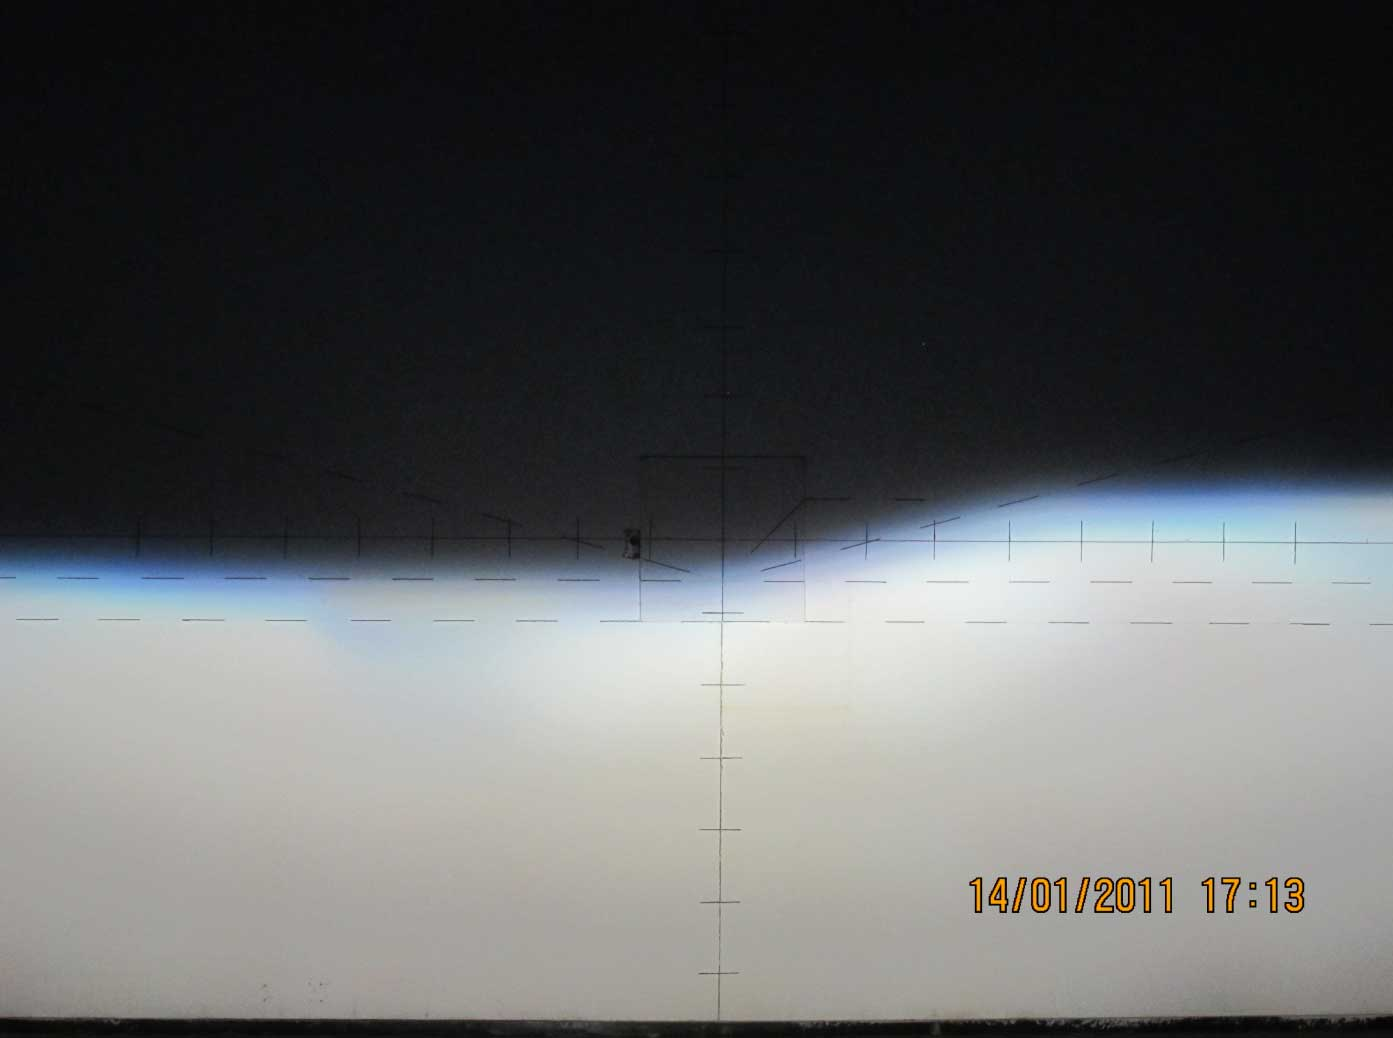
\includegraphics[width=10cm]{slike/original.jpg}
\end{center}
\caption{Vhodni parameter, sprednji žaromet.}
\label{pic:vhp1}
\end{figure}

\begin{figure}
\begin{center}
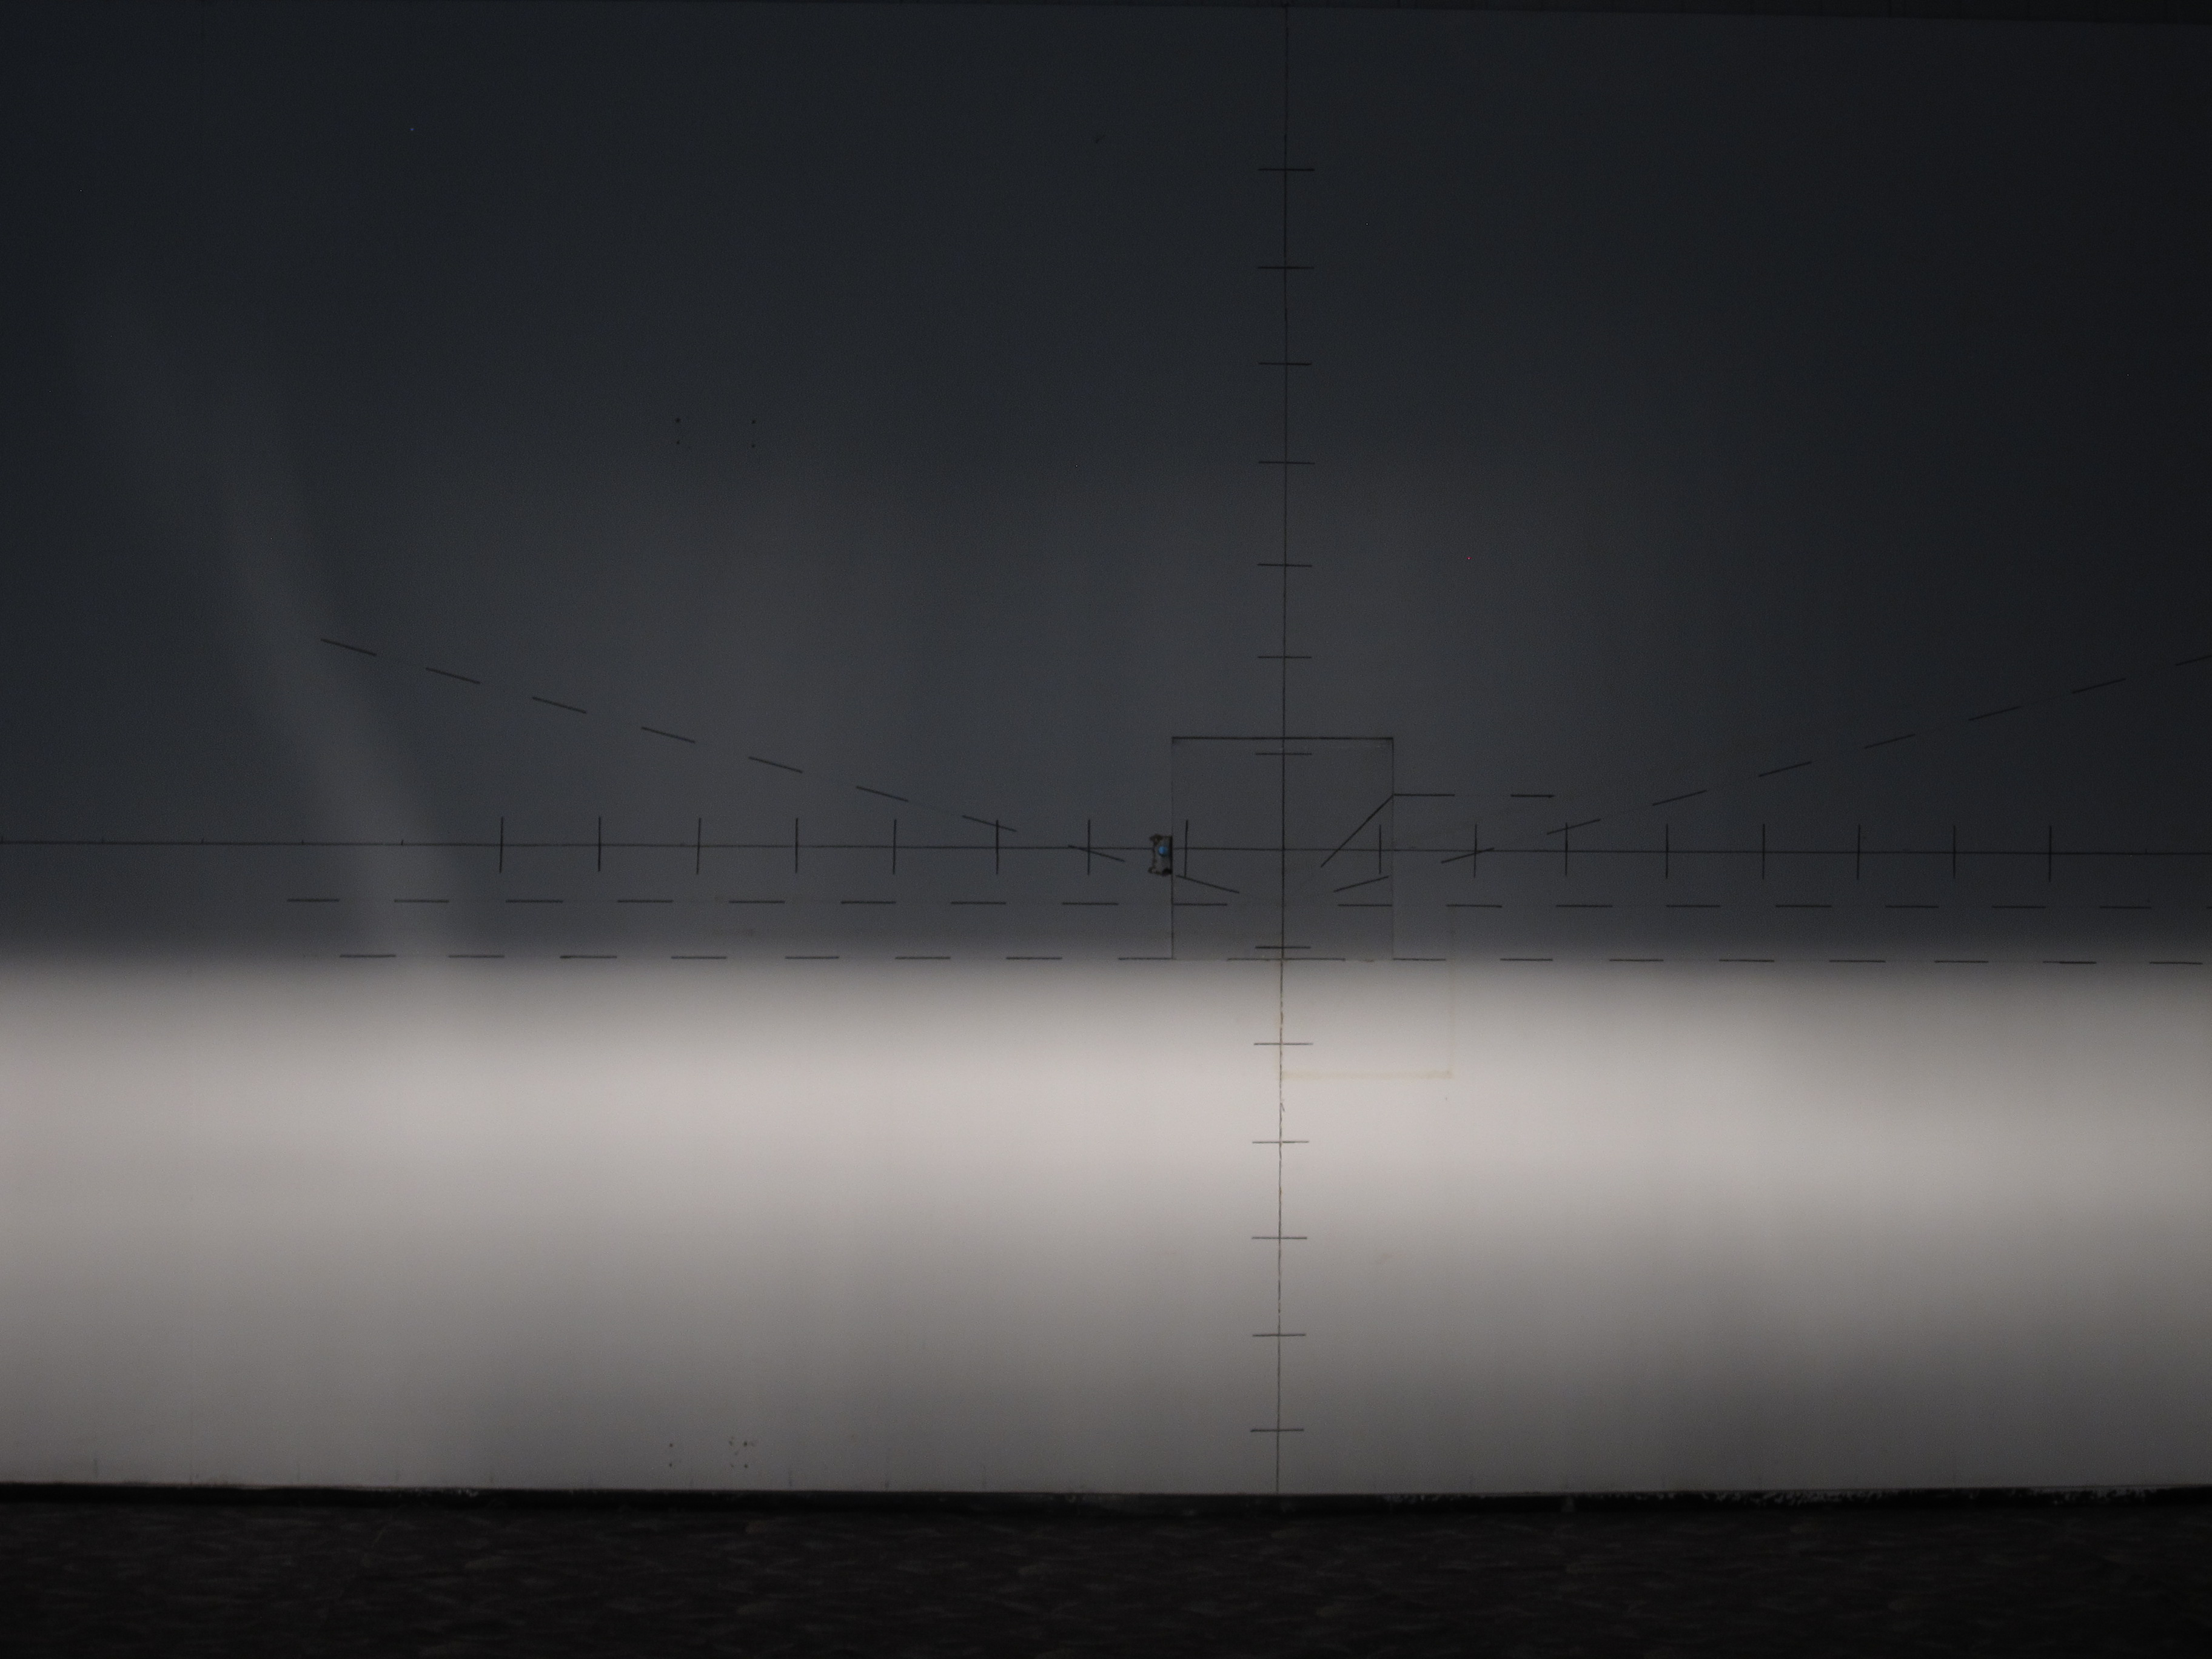
\includegraphics[width=10cm]{slike/levi3.JPG}
\end{center}
\caption{Vhodni parameter, meglenka.}
\label{pic:vhp2}
\end{figure}


\chapter{Sorodne rešitve}
\section{Fotometer}
Fotometer je naprava, ki jo v podjetju Hella Saturnus d.o.o. uporabljajo za določanje svetlobnih lastnosti žarometov. Žaromet se privije na optično os. Ta je nasproti fotocelici na razdalji petindvajset metrov. Za svetilke se uporablja razdalja tri metre. \\
Žarnice, ki se pri testih uporabljajo so različne od tistih v proizvodnji žarometov. Nitka v žarnici mora biti določene dolžine in je ne sme presegati za več kot milimeter. Daljša nitka lahko premakne svetlo-temno mejo.\\
Pri merjenju fotocelica stoji na miru. Premika se samo žaromet in sicer v vertikalni smeri. Na vsake 0,01 stopinje se pomeri svetilnost. Tako se ugotovi svetlo-temno mejo. Nahaja se kjer je največji gradient/razlika svetlobe med dvema točkama. Na razdalji 0,01 stopinje svetloba naraste za 20\%, pri kseon žarnicah tudi do 200\%.\\
Potem se preveri bleščanje žarometa, kjer se žaromet obrne tako da ne sveti v zaslon. Preveri pa se moč svetlobe (pod različnimi koti), ki pada na fotocelico.   \\
Standardi svetilnosti žarometov so od države do države različni. 

\chapter{Razvoj lastne aplikacije}
\section{Določitev strojne opreme}
Zahteve za delovanje programa:
\begin{itemize}
\item Prenosnik ali osebni računalnik.
\item Operacijski sistem Windows XP, Vista ali 7.
\item Instaliran .NET framework 4.0 ali več.
\item Intel ali Athlon procesor. 32 ali 64 biten. Priporočeno, da je več jedrni.
\item Priporočena količina pomnilnika je 2GB.
\item Velikost diska mora biti dovolj velika za operacijski sistem, .NET framework in slike svetlo-temnih mej. Sam program je velik par MB. 
\item Fotoaparat ali kamera (v načinu za slikanje ne snemanje).
\item Priporočena nastavitev fotoaparata za ISO je 100, slikanje s števcem ali stojalom.
\end{itemize}

\section{Uporabljene tehnologije}
Ena izmed zahtev naročnika programa je bila, da teče na operacijskem sistemu Windows. Pregledal sem več programskih jezikov, ki so na voljo za ta sistem. Moji glavni kriteriji so bili, da je programski jezik objektno usmerjen, da se v njem enostavno zgradi uporabniški vmesnik, in da zanj obstaja integrirano razvojno okolje. Pregledal sem jezike: Java, C\# .Net, Python, Delphi in PHP. Vsi jeziki so objektno usmerjeni, nekateri imajo dobro podporo za računalniški vid, nekateri nimajo avtomatičnega upravljanja s pomnilnikov... Spodaj so našteti dodatni plusi in minusi, ki sem jih ugotovil.

\subsection{Java}
\paragraph{Plusi}
\begin{itemize}
\item Sam skrbi za čiščenje pomnilnika.
\item Gradnja vmesnika v okolju Netbeans.
\item Knjižnica OpenCV za računalniški vid.
\end{itemize}
\paragraph{Minusi}
\begin{itemize}
\item Ne vsebuje standardnega uporabniškega vmesnika Windows.
\end{itemize}

\subsection{C\#}
\paragraph{Plusi}
\begin{itemize}
\item Sam skrbi za čiščenje pomnilnika.
\item Gradnja vmesnika v okolju Visual Studio.
\item Knjižnica Aforge za računalniški vid.
\item Knjižnice za paralelno procesiranje.
\item Knjižnica LINQ za enostavno delo s seznami in ostalimi podatkovnimi strukturami.
\end{itemize}


\subsection{Delphi}
\paragraph{Plusi}
\begin{itemize}
\item Standarden Windows uporabniški vmesnik.
\end{itemize}
\paragraph{Minusi}
\begin{itemize}
\item Slaba podpora za računalniški vid.
\end{itemize}

\subsection{Python}
\paragraph{Plusi}
\begin{itemize}
\item Sam skrbi za čiščenje pomnilnika.
\item Knjižnica OpenCV za računalniški vid.
\end{itemize}
\paragraph{Minusi}
\begin{itemize}
\item Slaba podpora za grafični uporabniški vmesnik (starejše verzije GTK+ in QT knjižnic za operacijski sistem Windows kot za Linux).
\end{itemize}

\subsection{PHP}
\paragraph{Plusi}
\begin{itemize}
\item HTML vmesnik, ki zgleda isto v večini operacijskih sistemov.
\end{itemize}
\paragraph{Minusi}
\begin{itemize}
\item Aplikacija bi morala biti v dveh delih. Uporabniški vmesnik, ki je napisan v PHP-ju in delu, ki bi procesiral slike.
\item Nima podpore za niti/paralelno procesiranje.
\item Slaba podpora za računalniški vid.
\end{itemize}

Moja končna izbira je bil C\#. Veliko zaradi osebnih preferenc. V njem sem najbolj domač. Visual Studio je zelo dobro integrirano okolje, ki omogoča hiter razvoj aplikacij. Vsebuje tudi dosti pripomočkov za pisanje kode. 
Uporabil sem knjižnico za računalniški vid Aforge .Net, predvsem zaradi hitrega delovanja, že implementiranih algoritmov za Sobelov in Hough-jev filter.
Za hranjenje kode sem uporabil sistem GIT, ki beleži zgodovino sprememb. Ima dobro podporo za vejanje in združevanje kode. Je enostaven in hiter za uporabo.


\section{Zasnova uporabniškega vmesnika}
Uporabniški vmesnik je razdeljen v osem glavnih sklopov. Te so originalna slika, črno-bela slika, Sobelov filter, prag, vodilne črte, vertikalne jakosti, svetlo-temna meja in širina svetlo-temne meje. Vsaka izmed teh je dosegljiva preko zavihkov (slika \ref{pic:vmesnik1}).

\begin{figure}
\begin{center}
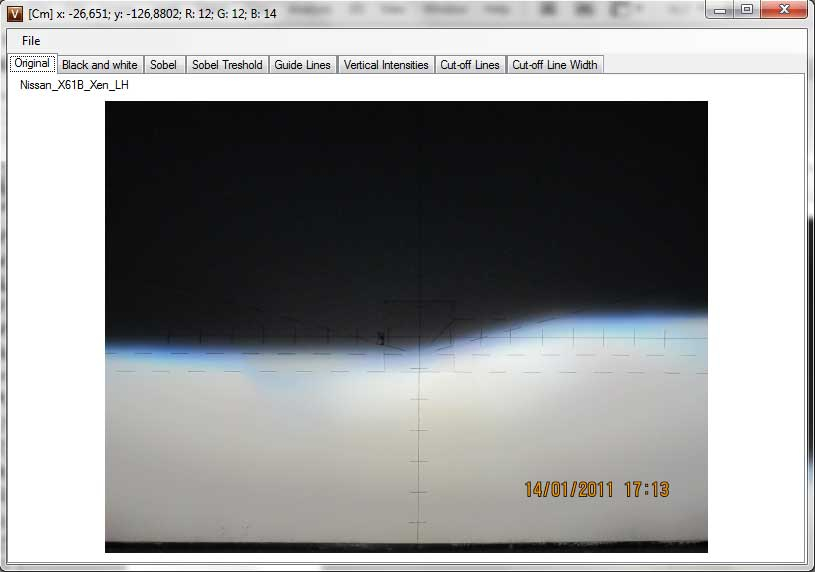
\includegraphics[width=10cm]{slike/vmesnik-glavni.jpg}
\end{center}
\caption{Uporabniški vmesnik programa.}
\label{pic:vmesnik1}
\end{figure}

\subsection{Vtičniki}

Vmesnik je zasnovan na principu vtičnikov [4, 5]. Vsak zavihek je svoj vtičnik in vsak ima svoj uporabniški vmesnik za konfiguracijo nastavitev. Definirani so s pomočjo vmesnika, ki zgleda tako:

\begin{verbatim}
interface IImagePlugin {
    UserControl UserInterface { get; }
    string Name { get; }
    bool ValidateInput();
    void ProcessImage();
}
\end{verbatim}
Lastnost UserInterface vrne uporabniški vmesnik vtičnika. Ta je lahko standarden s sliko na levi strani in konfiguracijskimi polji in gumbi na desni strani (slika \ref{pic:vmesnik2}). Lahko pa vsebuje samo graf (slika \ref{pic:vmesnik3}).


\begin{figure}
\begin{center}
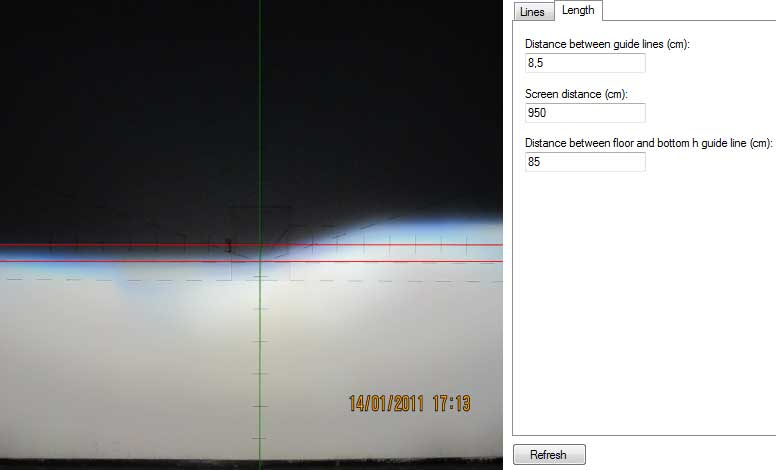
\includegraphics[width=10cm]{slike/vmesnik-slika-konfiguracija.jpg}
\end{center}
\caption{Primer uporabniškega vmesnika za iskanje vodilnih črt.}
\label{pic:vmesnik2}
\end{figure}

\begin{figure}
\begin{center}
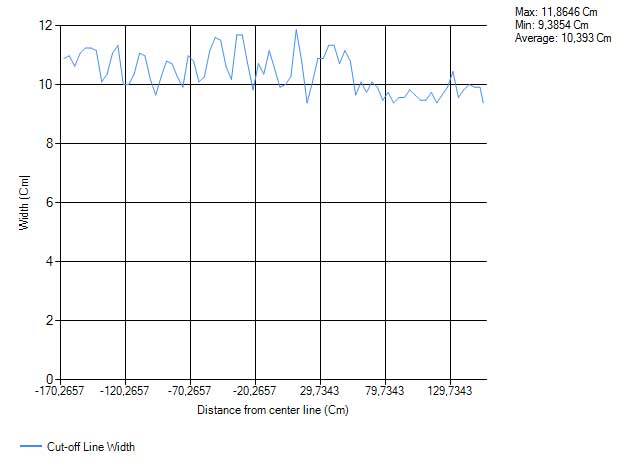
\includegraphics[width=10cm]{slike/vmesnik-samo-graf.jpg}
\end{center}
\caption{Primer uporabniškega vmesnika z grafom.}
\label{pic:vmesnik3}
\end{figure}

Funkcija ValidateInput se kliče, ko uporabnik pritisne gumb Refresh. Ta funkcija preveri vse vrednosti v poljih vmesnika, če imajo pravilno vsebino (če je podana širina število, da ni preveliko ali premajhno...). Funkcija ProcessImage se kliče po funkciji ValidateInput. Namenjena je procesiranju in obdelavi slike. Pri vtičniku črno-bela slika ta funkcija spremeni originalno sliko v črno-belo. V vtičniku vodilne črte pa ta funkcija najde vertikalno in dve horizontalni vodilni črti na sliki. Lastnost Name je ime vtičnika, ki je prikazana v imenu zavihka.

\subsection{Nalaganje vtičnikov}
Vtičniki niso del glavnega programa. Vsak vtičnik se nahaja v svoji knjižnici, ki se ob zagonu programa dinamično naloži. V programu je določena mapa vtičnikov. Iz te mape se preko .Net knjižnic za Reflection [5] naložijo vse knjižnice. V vsaki knjižnici se poišče implementacijo vmesnika IimagePlugin. Naredi se objekt, iz katerega se prebere uporabniški vmesnik. Tega se doda v nov zavihek z imenom našega vtičnika. Nakoncu se poveže še OnClick dogodek refresh gumba s metodama Validate in ProcessImage. V psevdokodi to zgleda tako:
\begin{verbatim}
foreach (dll in files_from_dir(plugins))
    foreach (class in dll.get_classes())
        if (class.implements(IImagePlugin))
            o = createObject(class)
            t = new Tab(o.Name)
            t.refreshButton.onclick += (sender, e) => {
                if (o.Validate)
                    o.ProcessImage()
            }
            t.controls.add(o.UserInterface)
            tabs.add(t)
\end{verbatim}

\subsection{Publisher-Subscriber model}
Vtičniki morajo nekako komunicirati med sabo. Slabo pa je, če vedo eden za drugega. Pravilo je, da so čim bolj neodvisni. Za tak primer prav pride vzorec po imenu Publisher-Subscriber [4, 5]. Deluje na principu dogodkov. Pri tem modelu nekdo pošilja sporočila, ki lahko vsebujejo slike, mere, velikosti točk... Vsi, ki so prijavljeni na določeno sporočilo, ga prejmejo in obdelajo. Vsebuje dve funkciji:

\begin{verbatim}
class PubSub {
    void Publish<T>(T message);
    void Subscribe<T>(Action<T> callback);
}
\end{verbatim}

Subscribe funkcija sprejme kot parametra tip sporočila na katerega se prijavljamo. Callback parameter je pa referenca na funkcijo, ki se pokliče, ko nekdo objavi sporočilo s tem tipom. Publish metoda se kliče, ko nekdo hoče objaviti sporočilo tipa T.
Recimo, da vtičnik za originalno sliko naloži sliko v procesiranje. Ta potem kliče metodo Publish z objektom tipa OriginalPictureLoadedMessage, ki to sliko vsebuje. Naslednjemu vtičniku, ki je prijavljen na ta sporočila, se bo klicala callback metoda. Sliko bo pa dobil preko parametera v callback metodi. Ta vtičnik je v našem programu za pretvorbo v črno belo sliko. Po tem, ko sliko tudi sam pretvori ponovno kliče metodo publish s sporočilom tipa BlackAndWhiteImageMessage. Tega nato prejme naslednji vtičnik in tako naprej.

\section{Postopek}
\subsection{Črno-bela slika}
Prvi korak v postopku je pretvorba slike v črno belo. To storimo tako, da za vsako piko na sliki izračunamo novo vrednost po formuli \ref{eq:bw}.

\begin{equation}
L=\dfrac{1}{2}(M+m)
\label{eq:bw}
\end{equation}

Kjer je M največja vrednost izmed RGB komponent točke. Vsaka točka je določena s tremi vrednostmi. Vsaka določa količino barve. R je za rdečo, G za zeleno in B za modro barvo. Te vrednosti so lahko od 0 do 255. Na tak način lahko opišemo barv. Spremenljivka m je najmanjša vrednost izmed RGB komponent. L je nova vrednost točke za črno-belo sliko. 
Trenutni algoritem se da pohitriti s paralelnim računanjem točk. Tako bi, pri 4 jedrnem procesorju, v enem koraku, izračunali 4 ali več točk hkrati.
Rezultat tega koraka je slika \ref{pic:bw}.



\begin{figure}
\begin{center}
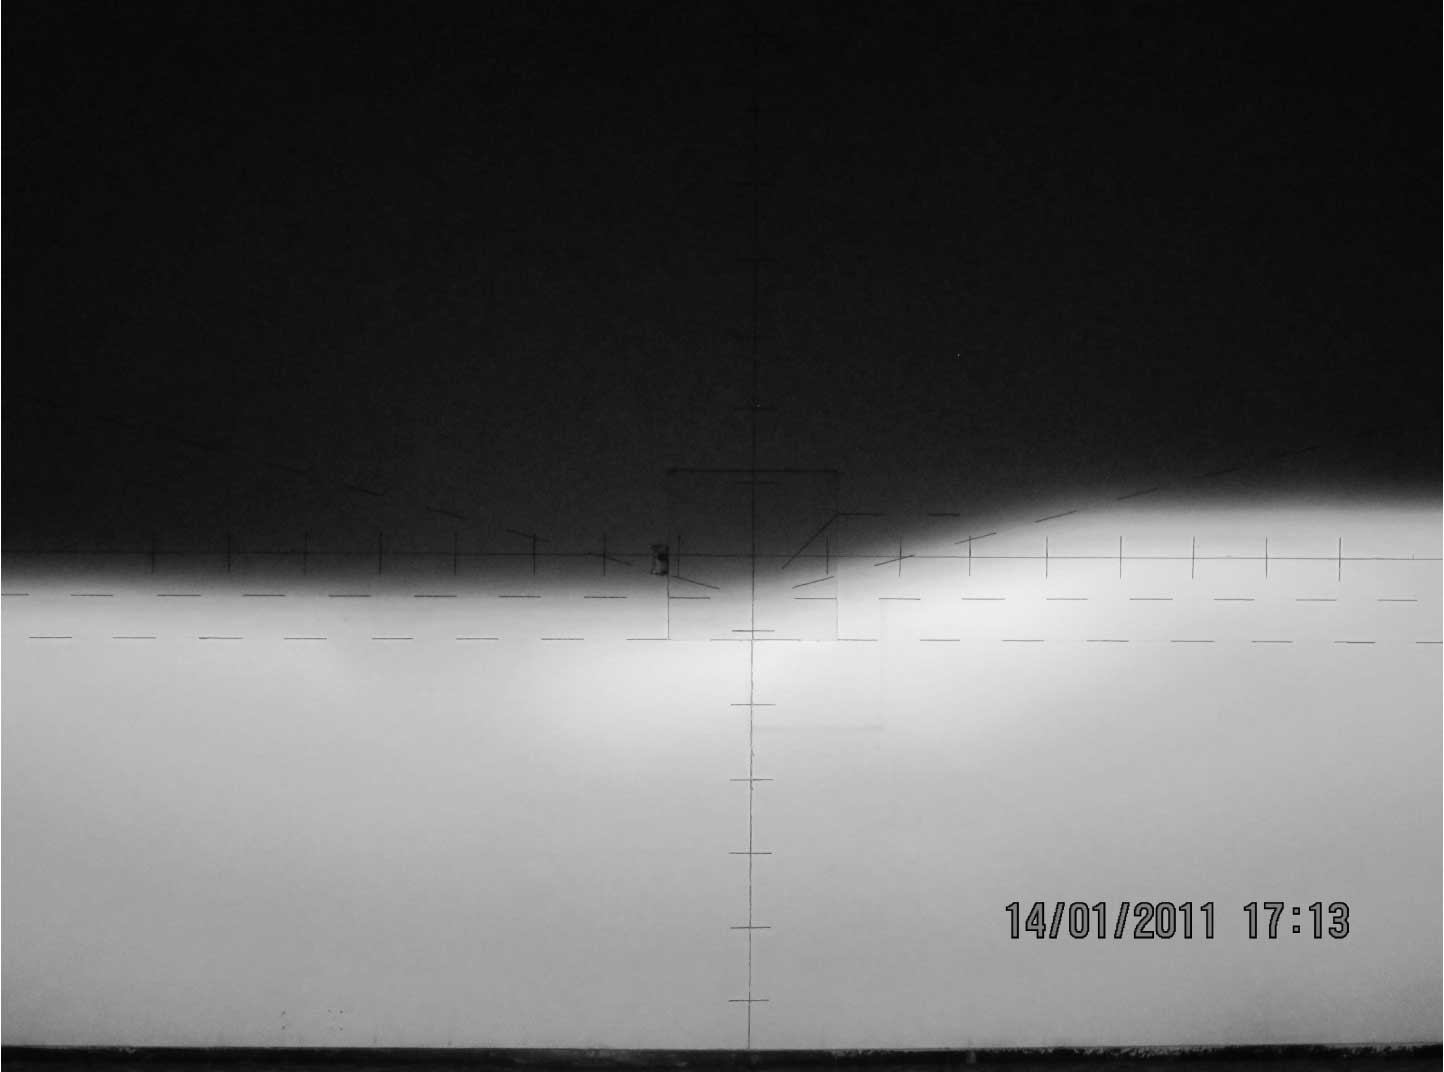
\includegraphics[width=10cm]{slike/crno-bela-slika.jpg}
\end{center}
\caption{Črno-bela slika.}
\label{pic:bw}
\end{figure}

\subsection{Sobelov filter}
Drugi korak v našem postopku je uporaba Sobelovega filtra. Ta nam pomaga kasneje pri odkrivanju  vodilnih črt na sliki. Tukaj je bila uporabljena knjižnica za računalniški vid Aforge.NET [1], kjer je ta filter že implementiran. Potreben je klic funkcije:
\begin{verbatim}
sobel = new SobelEdgeDetector().Apply(crnobelaslika);
\end{verbatim}

Rezultat filtra je slika \ref{pic:sobel}.

\begin{figure}
\begin{center}
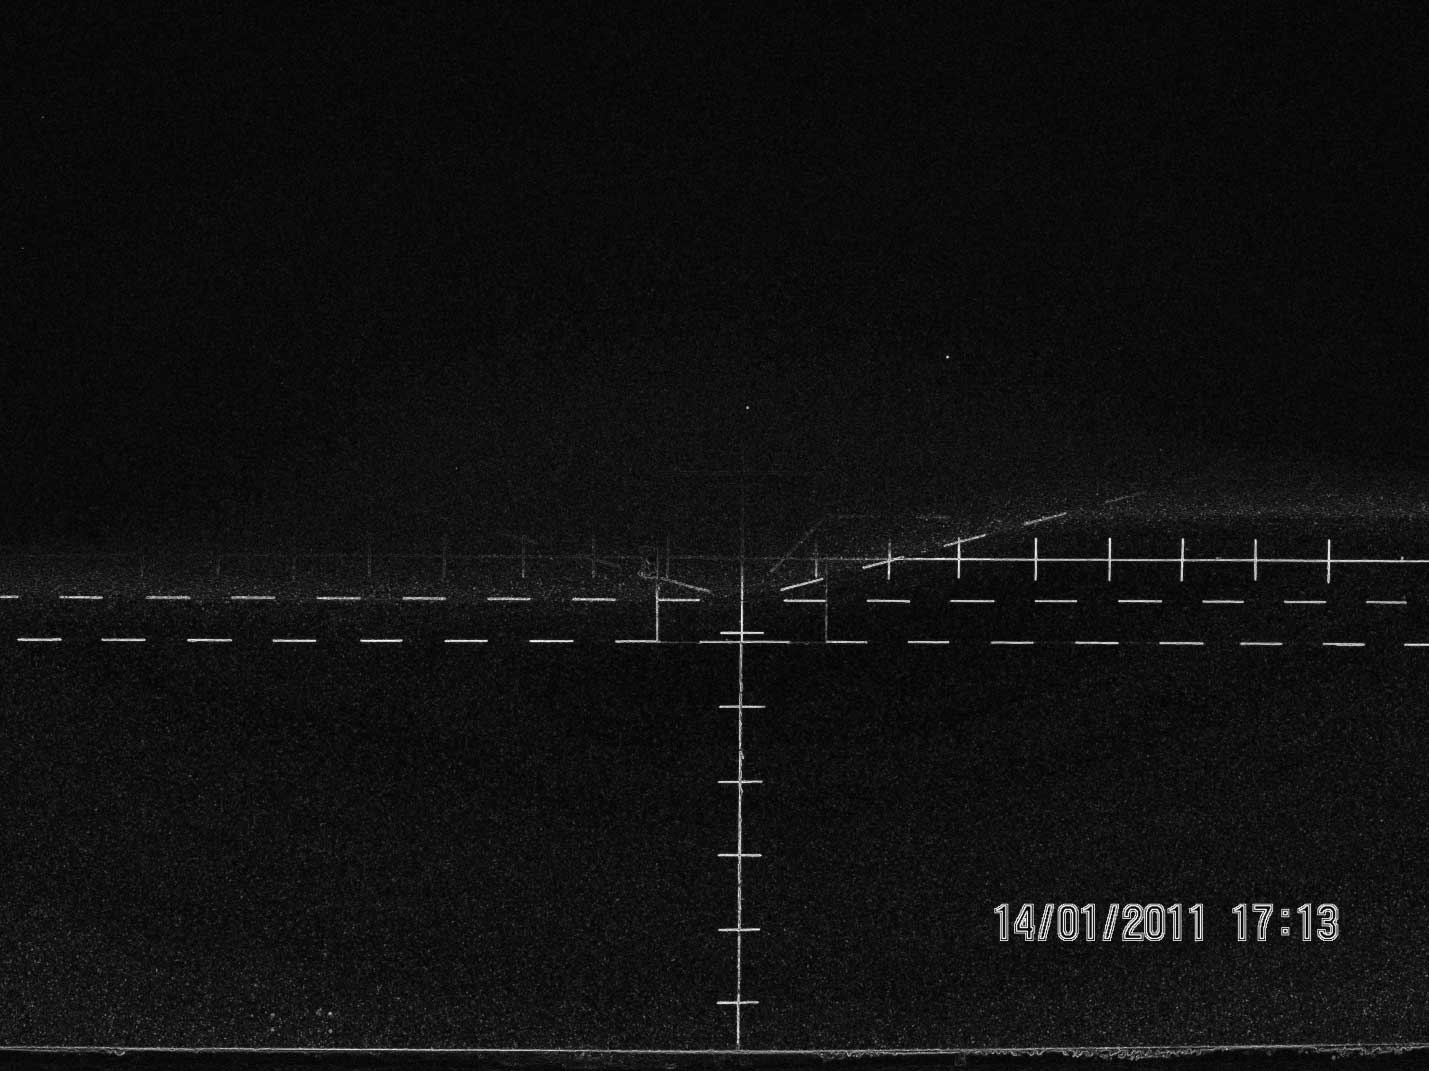
\includegraphics[width=10cm]{slike/sobel.jpg}
\end{center}
\caption{Sobelov filter.}
\label{pic:sobel}
\end{figure}

\subsection{Prag}
S tretjim korakom počistimo sliko iz poglavja Sobelov filter. To storimo tako, da za vsako točko pogledamo njeno intenziteto (pri pretvorbi v črno belo sliko imajo vse tri komponente točke isto vrednost). Intenziteta je enaka vrednosti ene izmed RGB komponent. Če je intenziteta večja od vrednosti, ki si jo uporabnik izbere (od 0 do 255), potem na novo sliko vpišemo točko z maksimalno intenziteto (bela pika). Če je ta vrednost manjša od izbrane, vpišemo črno piko. Tako na novi sliki še bolj poudarimo vodilne črte. In zmanjšamo količino šuma (točke, ki niso vodilne črte in ki bi ovirale njihovo detekcijo). Ta algoritem v psevdokodi izgleda tako:
\begin{verbatim}
for (int i = 0; i < visina(slika); i++)
    for (int j = 0; i < sirina(slika); j++)
        if (slika[i][j].R < prag)
            rezultat[i][j].R, G, B = 0
        else
            rezultat[i][j].R, G, B = 255
\end{verbatim}

Algoritem kot vhodni parameter sprejme bitno sliko in vrednost pragu. Kot rezultat pa vrne sliko \ref{pic:treshold}.

\begin{figure}
\begin{center}
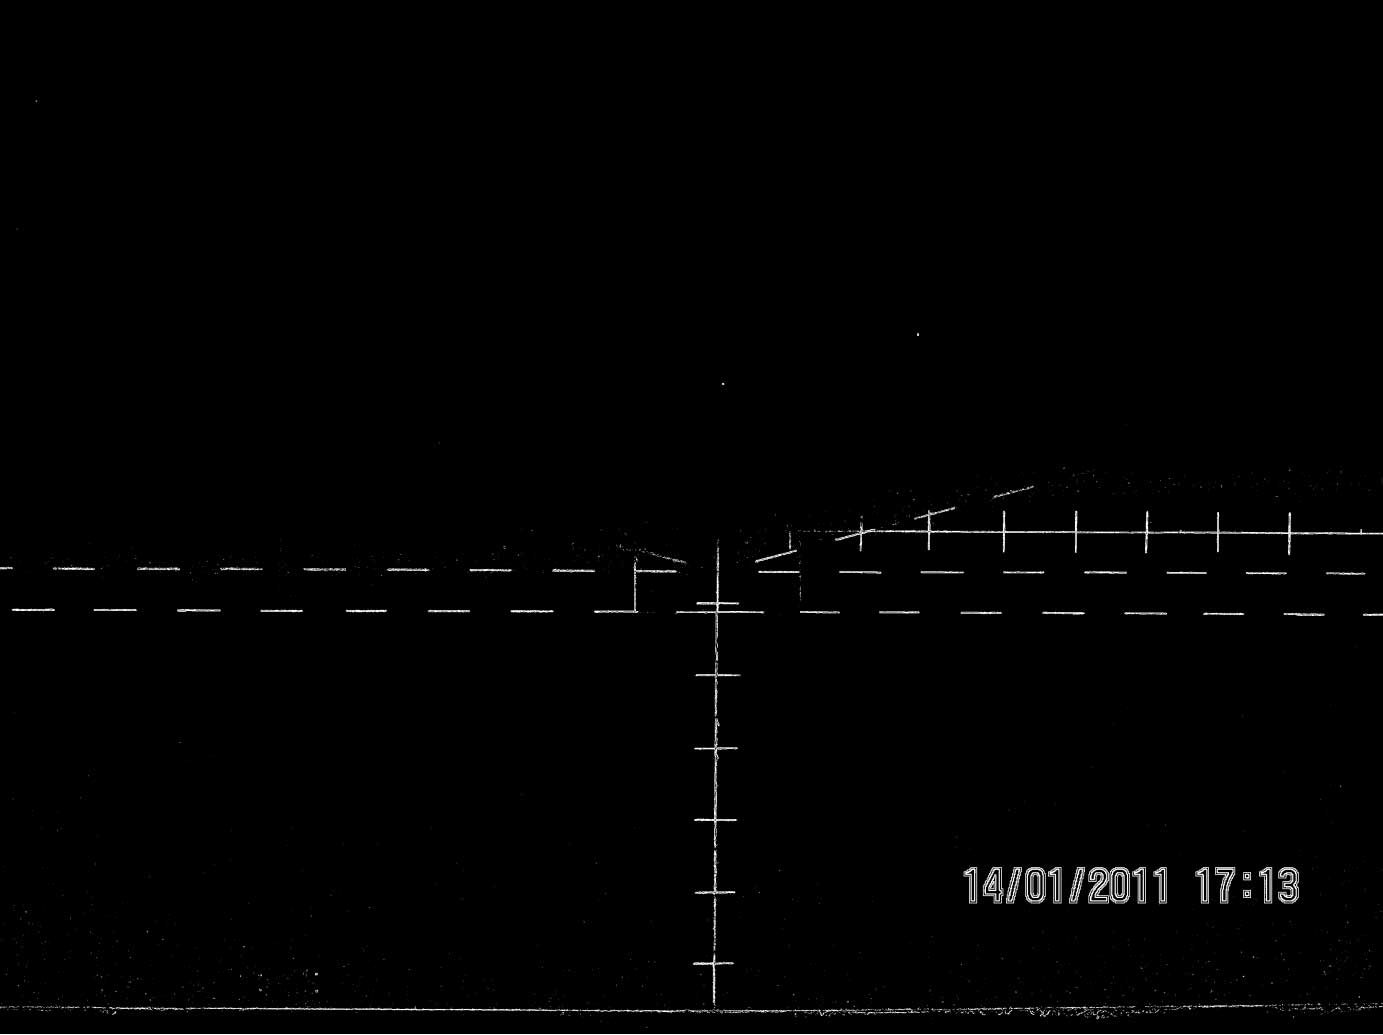
\includegraphics[width=10cm]{slike/treshold.jpg}
\end{center}
\caption{Prag.}
\label{pic:treshold}
\end{figure}


\subsection{Iskanje vodilnih črt}
V tem koraku iščemo prvi dve horizontalni vodilni črti (od zgoraj navzdol). In sredinsko vertikalno vodilno črto. Tukaj je uporabljena Hough-jeva črtna transformacija, ki se uporablja za detekcijo črt na sliki. Tudi ta je že implementirana v Aforge.NET knjižnici [2]. Primer klica za Hough-jevo transformacijo je:

\begin{verbatim}
HoughLineTransformation hlt = new HoughLineTransformation();
hlt.ProcessImage(sobel);
lines = hlt.GetLinesByRelativeIntensity(relativeIntensity);
IEnumerable<HoughLine> verticalLines = 
lines.Where(l => -5 <= l.Theta && l.Theta <= 5);
\end{verbatim}


Algoritem sprejme sliko pragu Sobelovega filtra. Vrne nam seznam črt, ki imajo večjo relativno jakost od parametra relativeIntensity [2] in kot med -5 in 5 stopinjami (s tem kotnim pogojem najdemo vertikalne črte, za horizontalne črte uporabimo kote od 85° do 95°). Relativna jakost črte je odvisna od števila belih pik, ki ležijo na črti. Vsaka črta je predstavljena z oddaljenostjo od centralne točke na sliki in kotom. Tako je recimo črta na oddaljenosti 0 in kotom 90 zelo blizu naše prve horizontalne črte, ki jo iščemo. Črta z oddaljenostjo 0 in kotom 0 stopinj pa blizu naše vertikalne vodilne črte [2]. 

\begin{figure}
\begin{center}
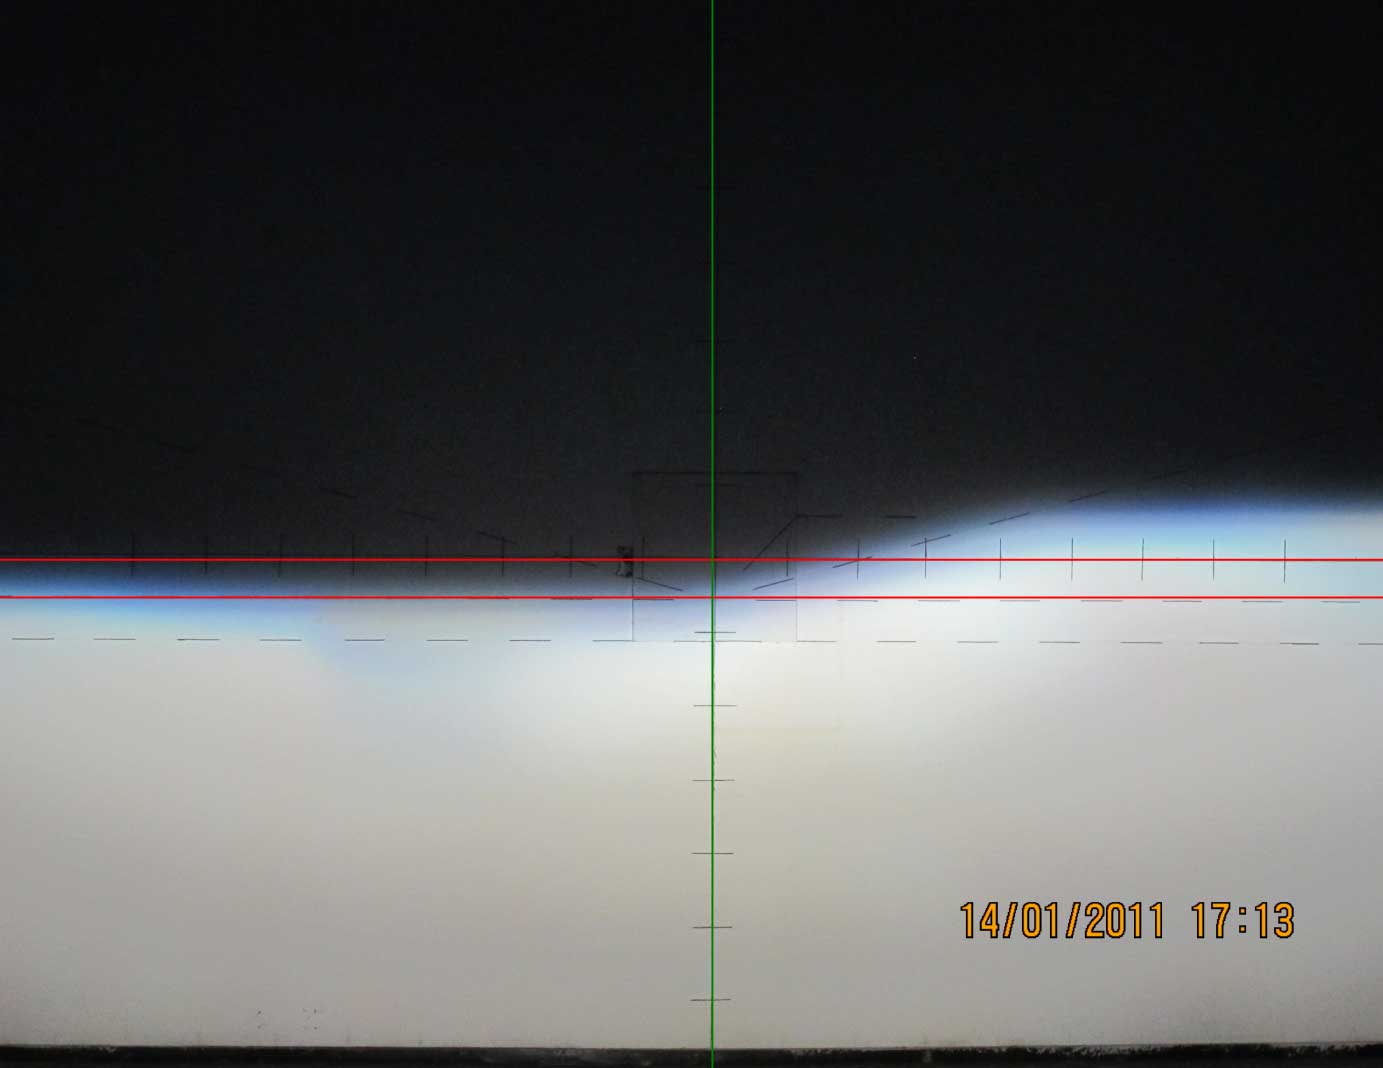
\includegraphics[width=10cm]{slike/vodilne-crte.jpg}
\end{center}
\caption{Vodilne črte.}
\label{pic:vodilne-crte}
\end{figure}

Te črte (slika \ref{pic:vodilne-crte}) se nato uporabijo za določitev mer na sliki (v kotih in centimetrih). Uporabnik vnese razdaljo med horizontalnima črtama in razdaljo od zaslona do kamere (v centimetrih). Iz tega lahko izračunamo koliko točk na sliki je en centimeter. Formula za izračun je formula \ref{eq:ps}.

\begin{equation}
v=\dfrac{a}{|r1-r2|}
\label{eq:ps}
\end{equation}


Kjer je v velikost točke v cm. Spremenljivka a je razdalja v cm med horizontalnima vodilnima črtama. R1 in r2 sta pa razdalji od centralne točke na sliki (v točkah).
Vsako točko na sliki lahko podamo tudi v kotu glede na centralno vertikalno ali horizontalno vodilno črto. Formula za izračun kota je formula \ref{eq:kot}.

\begin{equation}
tan(\alpha)=\dfrac{a}{b}
\label{eq:kot}
\end{equation}

A je oddaljenost, v cm, trenutne točke od centralne vodilne črte. B je oddaljenost zaslona od kamere. Alfa je kot, ki ga iščemo.

\subsection{Pregled intenzitet po vertikali}
Ta korak je glavni za določitev svetlo temne meje. To storimo tako, da izberemo vertikalo na sliki in pogledamo intenzitete njenih točk (0 do višine naše slike). Za sliko uporabimo črno belo sliko iz prvega koraka. Intenzitete nato izrišemo na grafu (slika \ref{pic:intenzitete1} in slika \ref{pic:intenzitete2}).

\begin{figure}
\begin{center}
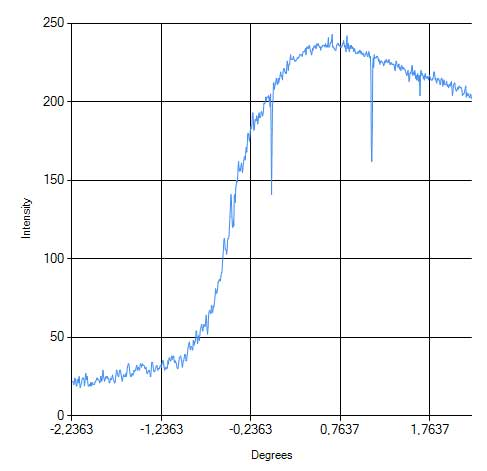
\includegraphics[width=10cm]{slike/intenzitete.jpg}
\end{center}
\caption{Intenzitete v stopinjah.}
\label{pic:intenzitete1}
\end{figure}

\begin{figure}
\begin{center}
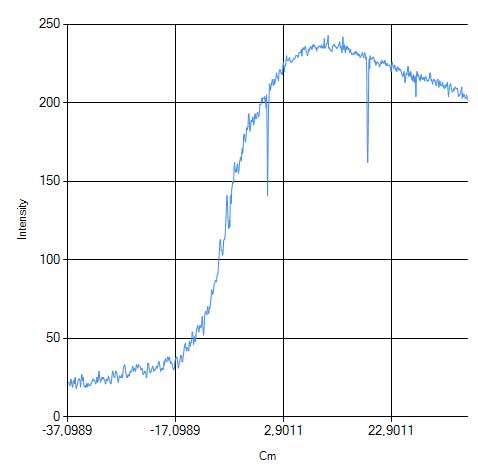
\includegraphics[width=10cm]{slike/intenzitete-v-cm.jpg}
\end{center}
\caption{Intenzitete v centimetrih.}
\label{pic:intenzitete2}
\end{figure}

Os x grafu slika \ref{pic:intenzitete1} predstavlja oddaljenost v stopinjah (\ref{pic:intenzitete2} v cm), od horizontalne vodilne črte. Na y osi je prikazana intenziteta točke. Primer tega algoritma v psevdokodi zgleda tako:


\begin{verbatim}
for (int i = 0; i < visina(slika); i++)
    vrednost = slika[i][x].R
    rezulat.dodaj(new XY(pretvori(i, enota), vrednost))
\end{verbatim}

Algoritem sprejme kot vhodni parameter sliko svetlo-temne meje. Prebere iz trenutne vrstice z indeksom i vrednost (intenziteta) v stolpcu x (naša vertikala). Pretvori koordinate vrstice i v izbrano enoto (stopinje ali centimetri). Na koncu shrani intenziteto in koordinate vrstice v seznam XY parov.

\subsection{Iskanje svetlo-temne meje}
Za svetlo temno mejo vzamemo prevojno točko na grafu. Ta točka se nahaja kjer je drugi odvod funkcije 0. Za izračun drugega odvoda uporabimo formulo \ref{eq:d2}.

\begin{equation}
d2=f(x+1) - 2f(x) + f(x-1)
\label{eq:d2}
\end{equation}

Kjer je f(x+1) naslednja točka na funkciji, f(x) trenutna in f(x-1) prejšnja točka. Funkcijo predstavimo s seznamom parov (X in Y) vrednosti tipa double. Pari so urejeni naraščajoče po vrednosti Y. Algoritem za izračun sprejme kot parameter našo funkcijo (spremenljivka f spodaj), vrne pa funkcijo drugega odvoda (d). Začnemo na drugem elementu v našem seznamu (zato, ker formula potrebuje prejšnji element). Končamo na predzadnjem elementu (ker formula potrebuje zadnji element).

\begin{verbatim}
For (i = 1; i < dolzina(f) – 1; i++) 
    d.dodaj(new XY(f[i + 1].X – 2 * f[i].X + f[i-1].X, f[i].Y))
\end{verbatim}

Slika \ref{pic:d2} prikazuje rezultat algoritma. Iz nje težko določimo katera ničla na grafu je prava. Originalna funkcija vsebuje veliko šuma. Dosti spreminja smer in tako vsebuje veliko prevojnih točk. Ta problem rešimo tako, da našo originalno funkcijo zgladimo z algoritmom za glajenje funkcij.


\begin{figure}
\begin{center}
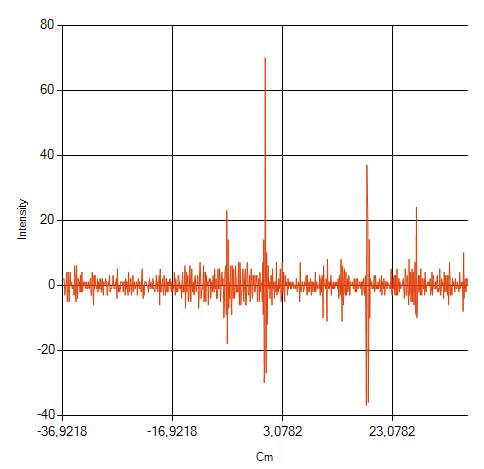
\includegraphics[width=10cm]{slike/drugi-odvod-1.jpg}
\end{center}
\caption{Drugi odvod funkcije.}
\label{pic:d2}
\end{figure}

\subsection{Glajenje funkcije}
V našem programu funkcijo gladimo tako, da jo povprečimo. Velikost okna (okno je število elementov, ki jih vzamemo v povprečje, ko računamo trenutni element) je nastavljiva s strani uporabnika. Obstaja več načinov kako povprečiti funkcijo. V povprečje lahko upoštevamo samo elemente pred trenutnim, lahko samo elemente za trenutnim. Najbolje se odnese, če vzamemo polovico velikosti okna elementov pred trenutnim in polovico elementov za. Torej, če je naše okno veliko deset, začnemo s šestim elementom, k njemu prištejemo pet elementov pred njim in pet za njim. Število, ki ga dobimo delimo s enajst in to je naš rezultat za trenutni element. Nadaljujemo dokler nam elementov/točk v naši originalni funkciji ne zmanjka. 

\begin{verbatim}
a = dolzina(f) / 2
for (i = a; i < dolzina(f) – a; i++)
    sum = 0
    for (j = i – a; j < i + a; j++)
        sum += f[j].X
    r.dodaj(new XY(sum / (a * 2 + 1), f[i].Y))
\end{verbatim}

Spremenljivka r je rezultat in zglajena funkcija našega algoritma (slika \ref{pic:smooth1} in slika \ref{pic:smooth2}).
Slika \ref{pic:smooth1} prikazuje našo zglajeno funkcijo. Slika \ref{pic:smooth2} pa prikazuje primerjavo med originalno in zglajeno funkcijo.

\begin{figure}
\begin{center}
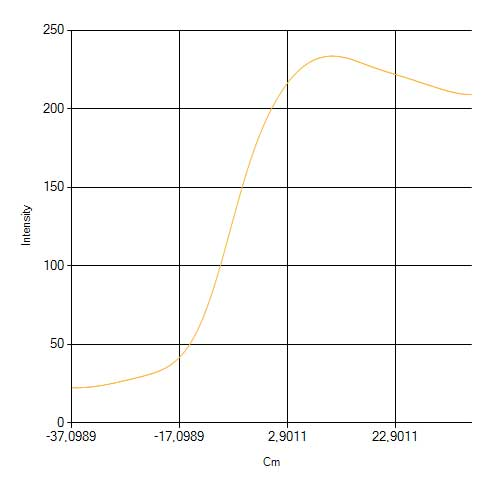
\includegraphics[width=10cm]{slike/glajena-funkcija.jpg}
\end{center}
\caption{Zglajena funkcija.}
\label{pic:smooth1}
\end{figure}

\begin{figure}
\begin{center}
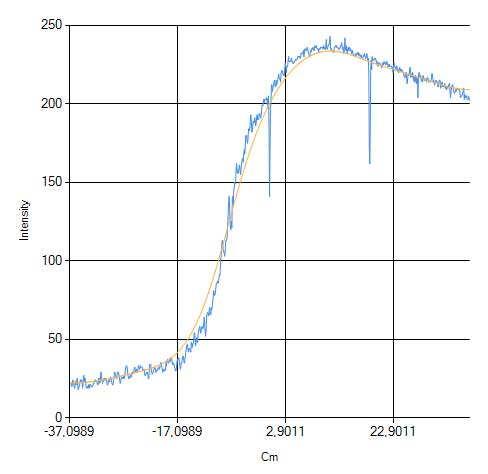
\includegraphics[width=10cm]{slike/glajena-+-original.jpg}
\end{center}
\caption{Primerjava zglajene in originalne funkcije.}
\label{pic:smooth2}
\end{figure}

Če sedaj to zglajeno funkcijo (slika \ref{pic:smooth1}) še enkrat odvajamo, dobimo lepšo funkcijo drugega odvoda (slika \ref{pic:d22}, kjer lahko določimo točko svetlo-temne meje.

\begin{figure}
\begin{center}
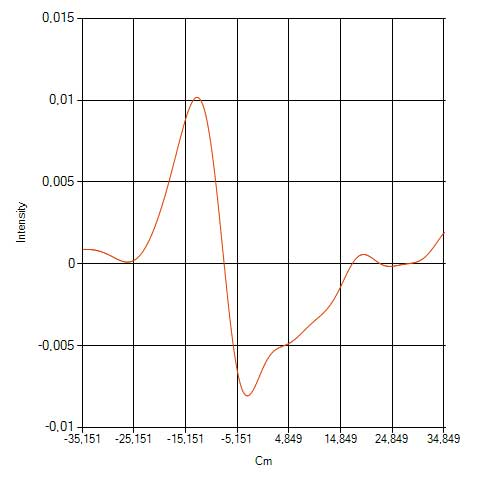
\includegraphics[width=10cm]{slike/drugi-odvod-2.jpg}
\end{center}
\caption{Drugi odvod zglajene funkcije.}
\label{pic:d22}
\end{figure}






\chapter{Sklicevanje na besedilne konstrukte}
\label{ch1}
Matematična ali popolna indukcija je eno prvih orodij, ki jih spoznamo za dokazovanje trditev pri matematičnih predmetih. 
\begin{izrek}
\label{iz:1}
Za vsako naravno število $n$ velja
\begin{equation}
n < 2^n.
\label{eq:1}
\end{equation}
\end{izrek}
\begin{dokaz}
Dokazovanje z indukcijo zahteva, da neenakost~\eqref{eq:1} najprej preverimo za najmanjše naravno število --- $0$. Res, ker je $0 < 1 = 2^0$, je neenačba~\eqref{eq:1} za $n=0$ izpolnjena.

Sledi indukcijski korak. S predpostavko, da je neenakost~\eqref{eq:1} veljavna pri nekem naravnem številu $n$, je potrebno pokazati, da je ista neenakost v veljavi tudi pri njegovem nasledniku --- naravnem številu $n+1$. Računajmo.
\begin{align}
n+1 &< 2^n + 1  \label{eq:2}\\
    &\le 2^n + 2^n \label{eq:3}\\
    &= 2^{n+1} \nonumber
\end{align} 
Neenakost~\eqref{eq:2} je posledica indukcijske predpostavke, neenakost~\eqref{eq:3} pa enostavno dejstvo, da je za vsako naravno število $n$ izraz $2^n$ vsaj tako velik kot 1. S tem je dokaz Izreka~\ref{iz:1} zaključen.
\end{dokaz}

Opazimo, da je \LaTeX\ številko izreka podredil številki poglavja.


\chapter{Plovke: slike in tabele}
\label{ch2}
Slike in daljše tabele praviloma vključujemo v dokument kot plovke. Pozicija plovke v končnem izdelku ni pogojena s tekom besedila, temveč z izgledom strani. \LaTeX\ bo skušal plovko postaviti samostojno, praviloma na vrh strani, na kateri se na takšno plovko prvič sklicujemo. Pri tem pa bo na vsako stran končnega izdelka želel postaviti tudi sorazmerno velik del besedila. V skrajnem primeru, če imamo res preveč plovk, se bo odločil za stran popolnoma zapolnjeno s plovkami.

\section{Formati slik}
Bitne slike, vektorske slike, kakršnekoli slike, z \LaTeX{}om lahko vključimo vse. 
Slika~\ref{pic1} je v {\tt .pdf} formatu.
\begin{figure}
\begin{center}
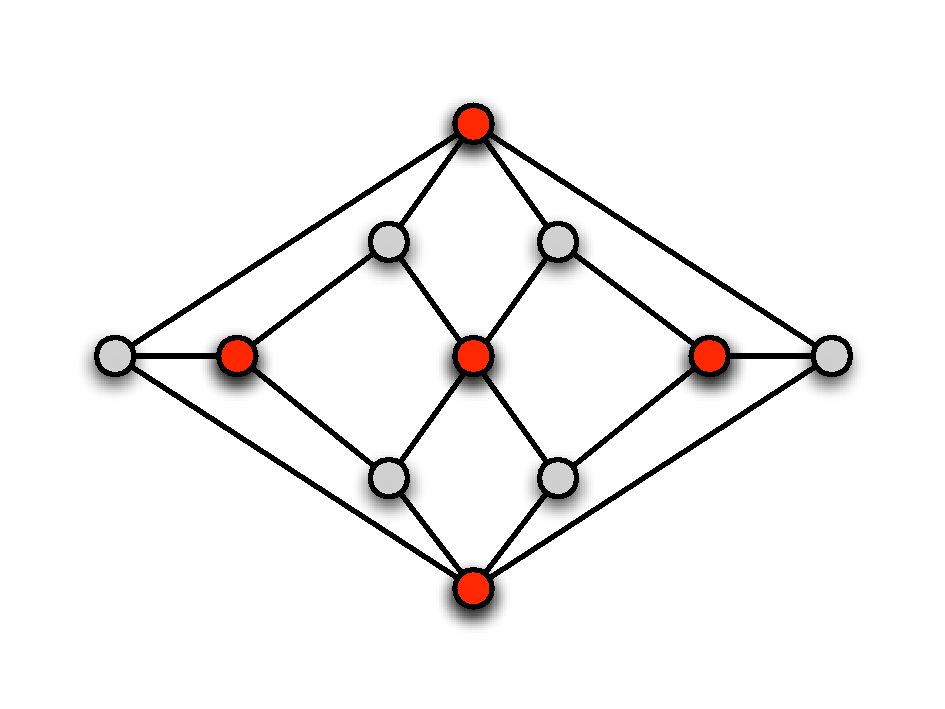
\includegraphics[width=10cm]{pic1.pdf}
\end{center}
\caption{Herschelov graf, vektorska grafika.}
\label{pic1}
\end{figure}
Pa res lahko vključimo slike katerihkoli formatov? Žal ne. Programski paket \LaTeX\ lahko uporabljamo v več dialektih. Ukaz {\tt latex} ne mara vključenih slik v formatu Portable Document Format {\tt .pdf}, ukaz {\tt pdflatex} pa ne prebavi slik v Encapsulated Postscript Formatu {\tt .eps}. 
Strnjeno v Tabeli~\ref{tbl:1}.

\begin{table}
\begin{center}
\begin{tabular}{l|ccc}
ukaz/format & {\tt .pdf} & {\tt .eps} & ostali formati \\ \hline
{\tt pdflatex} & da & ne & da \\
{\tt latex}   & ne & da  & da
\end{tabular}
\end{center}
\caption{}
\label{tbl:1}
\end{table}

Nasvet? Odločite se za uporabo ukaza {\tt pdflatex}. Vaš izdelek bo brez vmesnih stopenj na voljo v {.pdf} formatu in ga lahko odnesete v vsako tiskarno. Če morate na vsak način vključiti sliko, ki jo imate v {\tt .eps} formatu, jo vnaprej pretvorite v alternativni format, denimo {\tt .pdf}.

Včasih se da v okolju za uporabo programskega paketa \LaTeX\ nastaviti na kakšen način bomo prebavljali vhodne dokumente. Spustni meni na Sliki~\ref{pic2} odkriva uporabo \LaTeX{}a v njegovi pdf inkarnaciji --- {\tt pdflatex}.
\begin{figure}
\begin{center}

\includegraphics[width=10cm]{pic2.png}
\end{center}
\caption{Kateri dialekt uporabljati?}
\label{pic2}
\end{figure} 

Vključena Slika~\ref{pic2} je seveda bitna.

Kaj pa stran iz študentskega referata?\label{pp}
Tudi njo lahko vključimo v dokument. Toda ne kot plovko.
 

%\chapter{}

\chapter{Kaj pa literatura}
\label{ch3}
Kot smo omenili že v uvodu, je pravi način za citiranje literature uporaba \BibTeX{}a~\cite{bib}. 
Programski paket \LaTeX je prvotno predstavljen v priročniku~\cite{lat} in je v resnici nadgradnja sistema \TeX\ avtorja Donalda Knutha, znanega po denimo, če izpustim njegovo umetnost programiranja, Knuth-Bendixovem algoritmu~\cite{dk1}.

Vsem raziskovalcem s področja računalništva pa svetujem v branje mnenje L.\ Fortnowa~\cite{lf}.

\chapter{Zaključek}
Izbira \LaTeX\ ali ne \LaTeX\ je seveda prepuščena vam samim. Res je, da so prvi koraki v \LaTeX{}u težavni. Ta dokument naj vam služi kot začetna opora pri hoji.

\begin{thebibliography}{99}
\bibitem{lf} L.\ Fortnow, ``Viewpoint: Time for computer science to grow up'',
{\it Communications of the ACM}, št.\ 52, zv.\ 8, str.\ 33--35, 2009.
\bibitem{dk1} D.\ E.\ Knuth, P. Bendix. ``Simple word problems in universal algebras'', v zborniku: Computational Problems in Abstract Algebra (ur. J. Leech), 1970, str. 263--297.
\bibitem{lat} L.\ Lamport. {\it LaTEX: A Document Preparation System}. Addison-Wesley, 1986.
\bibitem{bib} O.\ Patashnik (1998) \BibTeX{}ing. 
Dostopno na:\\ http://ftp.univie.ac.at/packages/tex/biblio/bibtex/contrib/doc/btxdoc.pdf
\bibitem{licence} licence-cc.pdf. Dostopno na: 
\end{thebibliography}
\end{document}

